
\FloatBarrier

\section{Система Дуффинга} %  % {{{1 _DUFF_
\label{atu:sect:duff}

\LinkRef{
 duff: ASAU-12, 15. APIR-2009. DSMP-2016
  % ~/doc/tex/asau/asau12/atu/atu.tex
  % ~/doc/tex/asau/asau15/atu/atu.tex
}

\subsection{Определение системы и анализ её динамики} %  % {{{2

Рассмотрим нелинейную динамическую систему Дуффинга~\cite{magni_theory_dyn_chaos,atu_asau12}:

\begin{equation}
 \ddot{x} + c_0 \dot{x} + \alpha x + \beta x^3 = u(t) ,
\label{atu:eq:duff}
\end{equation}
%
или её же с сохранением физических размерностей:
%
\begin{equation}
 m \ddot{x} + \nu \dot{x} + k_1 x + k_3 x^3 = F(t) ,
\label{atu:eq:duff_phys}
\end{equation}

Здесь $m$ -- масса объекта,
$x(t)$ -- координата (выходной сигнал),
$u(t) = U_{in} \sin( \omega_{in} t ) $ -- внешняя возмущающая сила,
$ k_1 $ -- коэффициент линейной компоненты возвращающей силы,
$ k_3 $ -- коэффициент при нелинейной части,
$ \alpha $ -- безразмерный коэффициент линейной компоненты возвращающей силы,
 при $ \alpha >0 $ и отсутствии нелинейности определяет собственную частоту: ($\Omega_0^2 = \alpha $),
$ \nu $ и $ c_0$ -- размерный и безразмерный коэффициенты демпфирования,
$ \beta $ -- безразмерный коэффициент нелинейной части.

Идентифицируемый параметр $ \beta $ определяет нелинейные свойства системы.
Следует отметить, что  данная система проявляет хаотические свойства
только при малых значениях параметра \(c_0\). При большем
влиянии диссипативной составляющей система~(\ref{atu:eq:duff}) качественно
не отличается от линейной колебательной системы,
и для её идентификации применимы классические критерии.

% Остальные параметры:
% \(U_{in}=1\), \(\omega_{in}=1\),
% \(c_0 = 0.05\), \( \alpha = -1 \).

На рис.~\ref{atu:f:duff_phase_f_reg} приведены
расширенный фазовый портрет и спектр системы Дуффинга
в режиме сложно-периодических колебаний.
Следует отметить, что существуют условия, при которых добавка к гармоническому входному сигналу
шумоподобной составляющей может перевести систему в хаотический режим~\cite{atu_asau15}.

\begin{figure}[ht!]
\begin{center}
  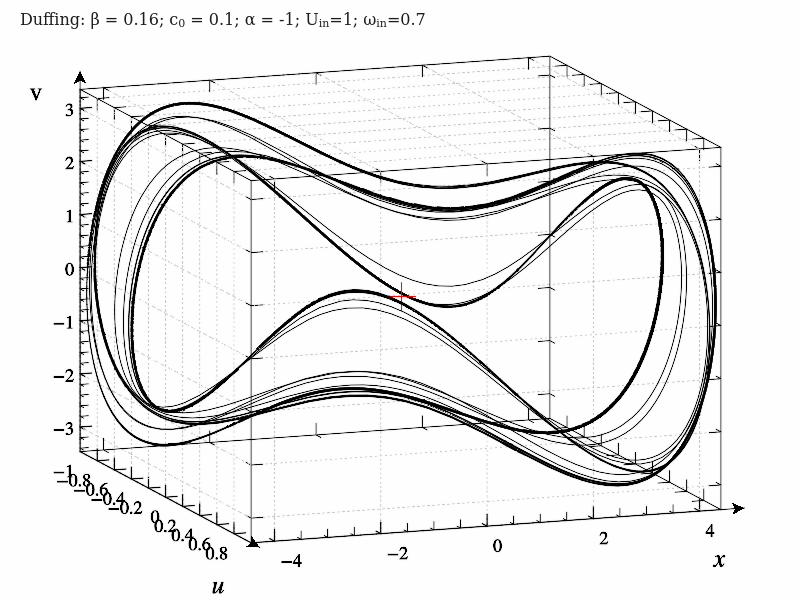
\includegraphics[width=0.49\textwidth]{p/cha/duff/duff_p_1x00_0x70_0x16.png}
  \hfill
  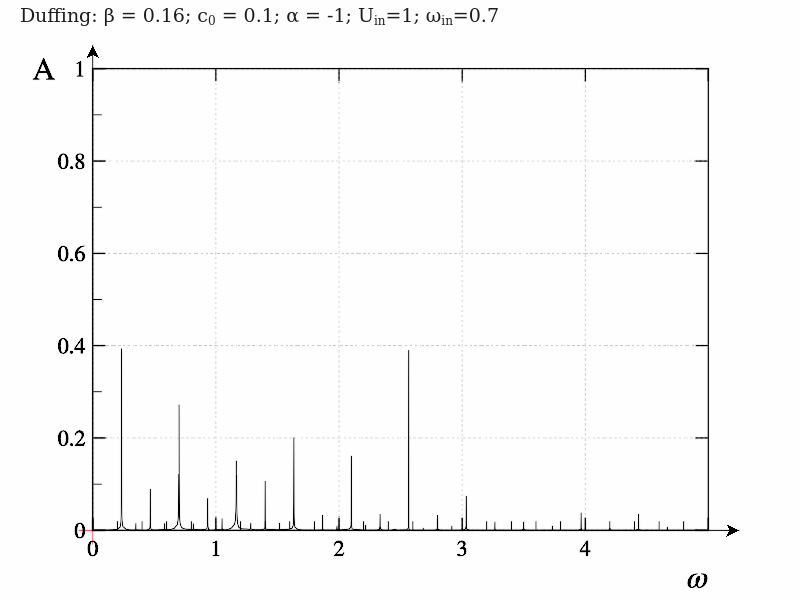
\includegraphics[width=0.49\textwidth]{p/cha/duff/duff_f_1x00_0x70_0x16.png}
\end{center}
  \caption{Расширенный фазовый портрет и спектр системы Дуффинга (\ref{atu:eq:duff}) в режиме сложно-периодических колебаний}
\label{atu:f:duff_phase_f_reg}
\end{figure}

Малые изменения параметра $\beta$ могут перевести систему в режим хаотических
колебаний, при которых вынуждающая частота отображается ярко выраженным пиком
(рис.~\ref{atu:f:duff_phase_f_chaos1}). Также выражены
третья и пятая гармоника входного сигнала,
а участок сплошного спектра выражен слабо.

\begin{figure}[ht!]
\begin{center}
  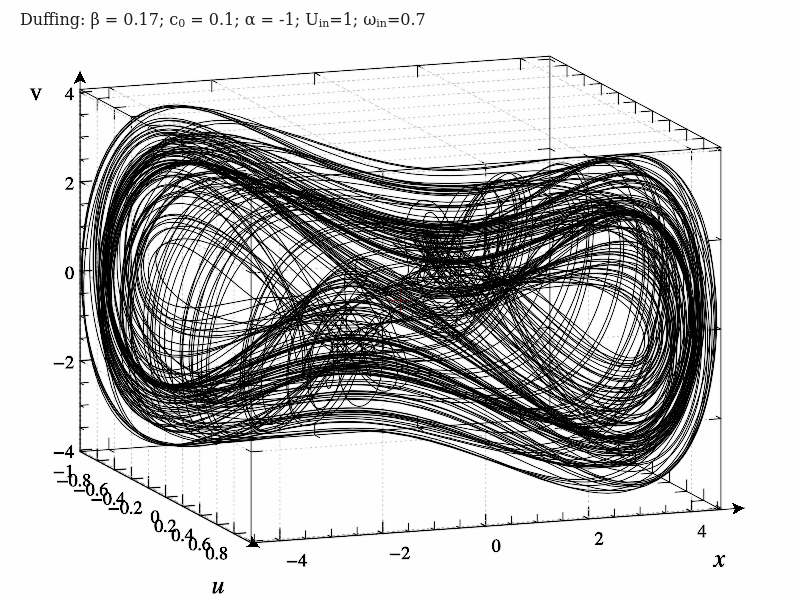
\includegraphics[width=0.49\textwidth]{p/cha/duff/duff_p_1x00_0x70_0x17.png}
  \hfill
  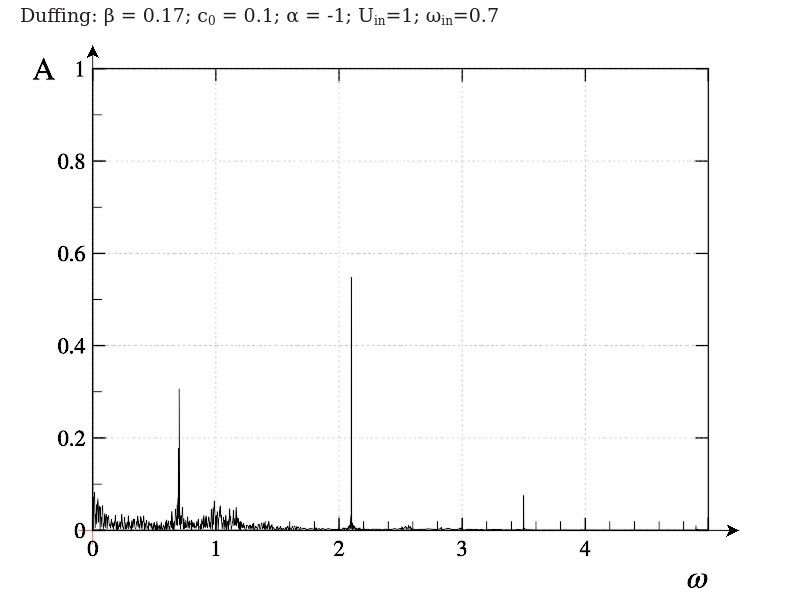
\includegraphics[width=0.49\textwidth]{p/cha/duff/duff_f_1x00_0x70_0x17.png}
\end{center}
  \caption{Расширенный фазовый портрет и спектр системы Дуффинга (\ref{atu:eq:duff}) в режиме слабо выраженных хаотических колебаний}
\label{atu:f:duff_phase_f_chaos1}
\end{figure}


При дальнейшем росте параметра $\beta$ происходит чередование хаотического
и сложно-периодического режимов. Наблюдаются участки,
на которых стабильно наблюдается хаотический режим,
при этом участки сплошного спектра выражены
сильнее~(рис.~\ref{atu:f:duff_phase_f_chaos2}).

\begin{figure}[ht!]
\begin{center}
  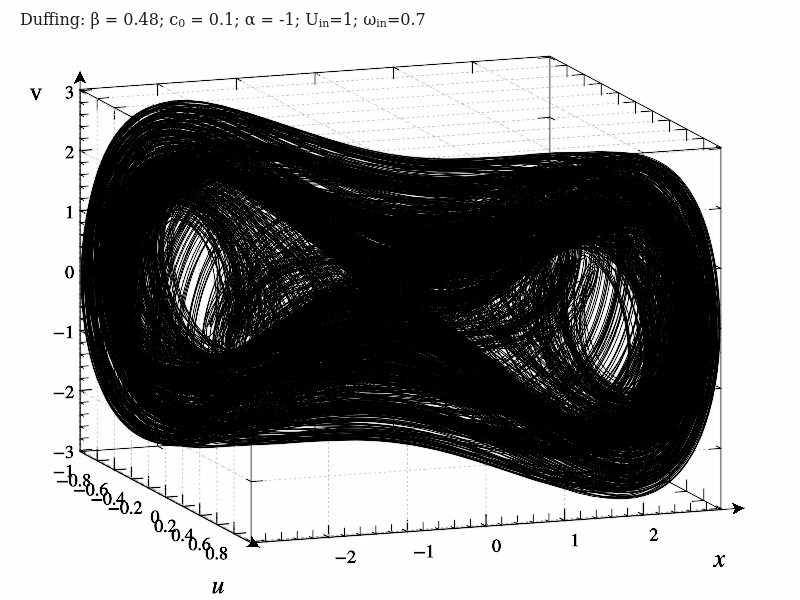
\includegraphics[width=0.49\textwidth]{p/cha/duff/duff_p_1x00_0x70_0x48.png}
  \hfill
  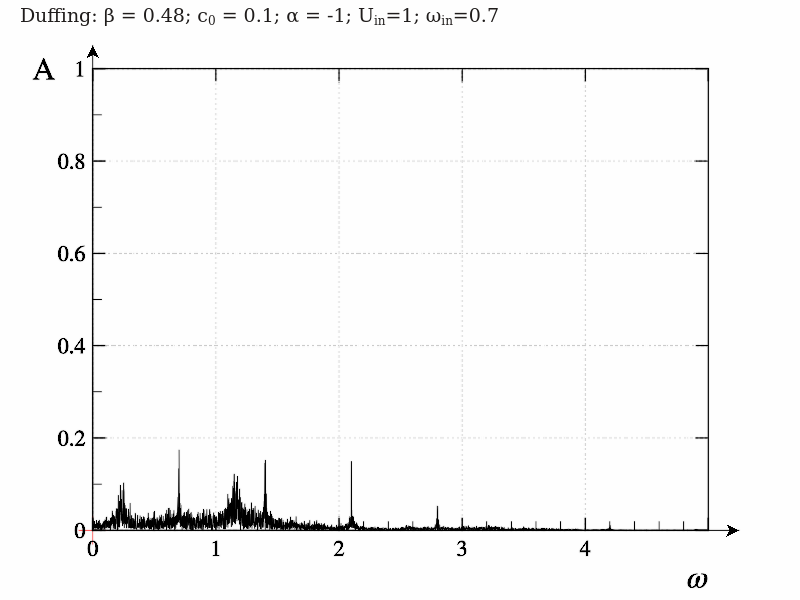
\includegraphics[width=0.49\textwidth]{p/cha/duff/duff_f_1x00_0x70_0x48.png}
\end{center}
  \caption{Расширенный фазовый портрет и спектр системы Дуффинга (\ref{atu:eq:duff}) в режиме выраженных хаотических колебаний}
\label{atu:f:duff_phase_f_chaos2}
\end{figure}


% \begin{figure}[htb!]
% \centerline{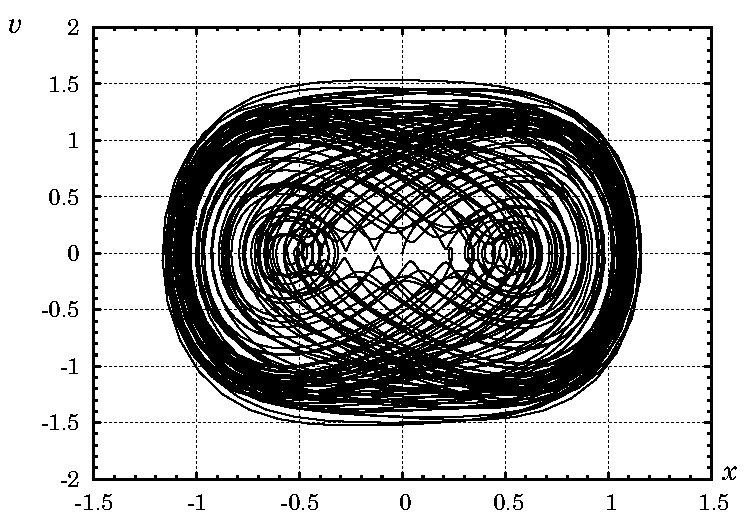
\includegraphics[width=0.5\textwidth]{p/cha/duff_phase.pdf} }
% \caption{Фазовый портрет системы Дуффинга (\ref{atu:eq:duff})}
% \label{atu:f:duff_phase}
% \end{figure}


% }}}2

\subsection{Анализ и выбор критерия}  % {{{2

Рассмотрим возможности определения вида критерия,
основываясь на физических принципах.
Исследуемая система из-за
малой величины \(c_0\) очень близка к консервативной,
и наблюдаемые изменения полной энергии системы
в основном обусловлены взаимодействием с внешним
источником энергии -- входным сигналом \(u(t)\).

Прежде всего отметим, что при неизменных параметрах
системы и входного сигнала, несмотря на то, что
система и её окружение постоянно обмениваются энергией,
среднее значение полной энергии системы остаётся постоянным.
В полную энергию вносят свой вклад кинетическая
%
\begin{equation}
E_k = m \frac{\dot{x}^2(t)}{2}
\label{atu:eq:duff_Ek}
\end{equation}
%
и потенциальная энергия
%
\begin{equation}
E_p = \int\limits_0^x ( k_1 x + k_3 x^3 ) dx =
\frac{k_1 x^2}{2} + \frac{k_3 x^4}{4}.
\label{atu:eq:duff_Ep}
\end{equation}

Как следует из (\ref{atu:eq:duff_Ep}), идентифицируемая
величина \( \beta \)
(в размерном виде ей соответствует параметр \(k_3\))
непосредственно входит только в выражение для
потенциальной энергии, причём её влияние играет большее
значения при максимальных значениях \(x(t)\).
Казалось бы, что в качестве величины, определяющей
критерий идентификации, можно было бы взять
максимальное значение выходного сигнала
при нулевом входе, так как при этом кинетическая энергия системы нулевая,
и создаются благоприятные условия для идентификации.
Однако, это достаточно редкие случаи, чтобы на их основе
строить надёжно работающую систему идентификации, и
естественно, возникает вопрос о точности измерений таких редких
событий.

Воспользуемся тем, что влияние параметра \(\beta\)
наиболее существенно при максимальных значениях \(x\),
и, следовательно, в первую очередь оказывает влияние на величину
%
\begin{equation}
 P = \frac{1}{\tau}\int\limits_0^\tau x^2(t) dt ,
\label{atu:eq:duff_P}
\end{equation}
%
где \(\tau\) -- достаточно большой интервал усреднения.
В свою очередь, данную величину просто измерять,
из-за большого значения \(\tau\) (обычно порядка нескольких десятков
периодов входного сигнала) влияние шумов измерения минимально.

Таким образом, в качестве критерия имеет смысл использовать
$q_{x^2}$, $q_{|x|}$. При этом, ввиду близкой к гиперболической зависимости
имеет смысл включить в рассмотрение и критерий $q_{x^{-2}}$.
Указанные зависимости, полученные при моделировании динамики системы~(\ref{atu:eq:duff})
представлены на рис.~\ref{atu:f:duff_q}.

\begin{figure}[ht!]
\begin{center}
  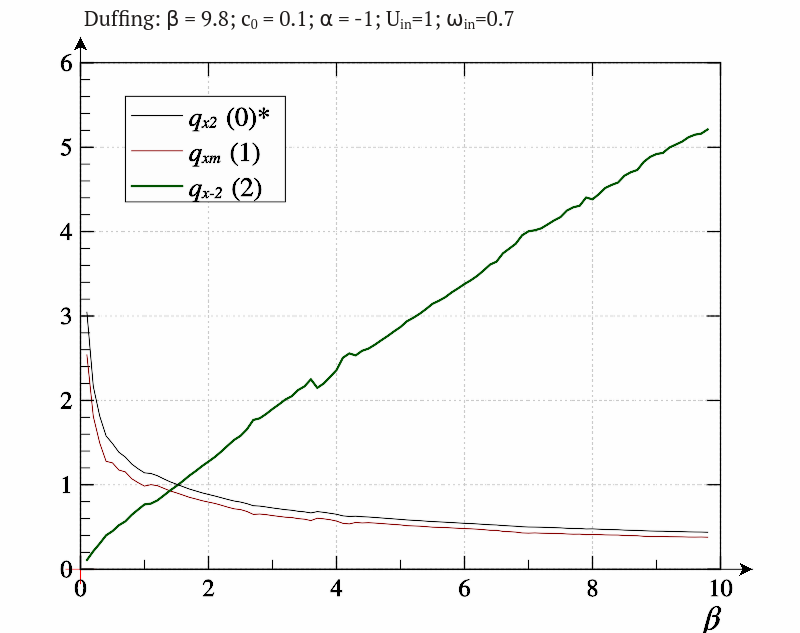
\includegraphics[width=0.49\textwidth]{p/cha/duff/duff_q-p_q_1x00_0x70.png}
\end{center}
  \caption{Зависимости $q_{x^2}(\beta)$, $q_{|x|}(\beta)$,  и $q_{x^{-2}}(\varepsilon) $ для системы Дуффинга}
\label{atu:f:duff_q}
\end{figure}

Анализ графиков позволяет сделать вывод, что критерий $q_{x^{-2}}$
наиболее подходит для проведения идентификации. При это наблюдаются
небольшие нарушения монотонности, что потенциально должно привести к
росту ошибки идентификации в окрестностях этих нарушений.



% }}}2

\subsection{Тестовая задача идентификации для системы Дуффинга}  % {{{2

При синтеза системы идентификации использовалась группа методов ``ql3rlWvnAAW''
при использовании критерия $q_{x^{-2}}$.
Значений параметров выбирались так, что бы обеспечить
наличие всех видов колебаний в рабочем диапазоне:
$U_{in}=1.0$, $\omega_{in}=0.7$, $ \beta \in [1, 4]$.

Рассмотрим процесс идентификации
в квазистационарном случае,
при медленном изменении параметра~(\ref{atu:eq:po_t_ramp}), $p_0=1$, $U_p=2$.
Динамика агентов и различных способов задания $p_\mathrm{id}$
представлена на рис.~\ref{atu:f:duff_id_ramp}.

\begin{figure}[ht!]
\begin{center}
  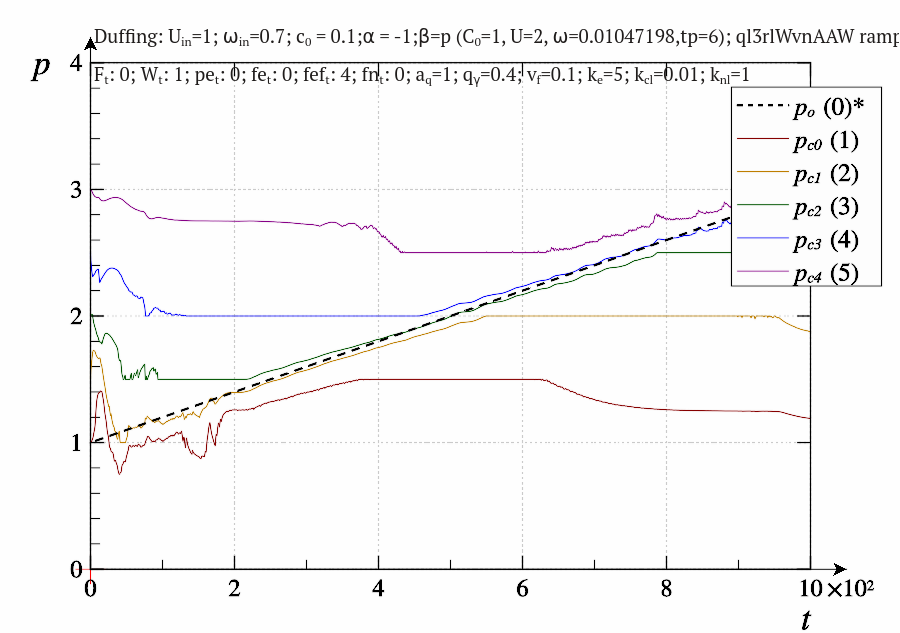
\includegraphics[width=0.49\textwidth]{p/cha/duff/duff_id-p_t_pi_ql3rlWvnAAW_ramp.png}
  \hfill
  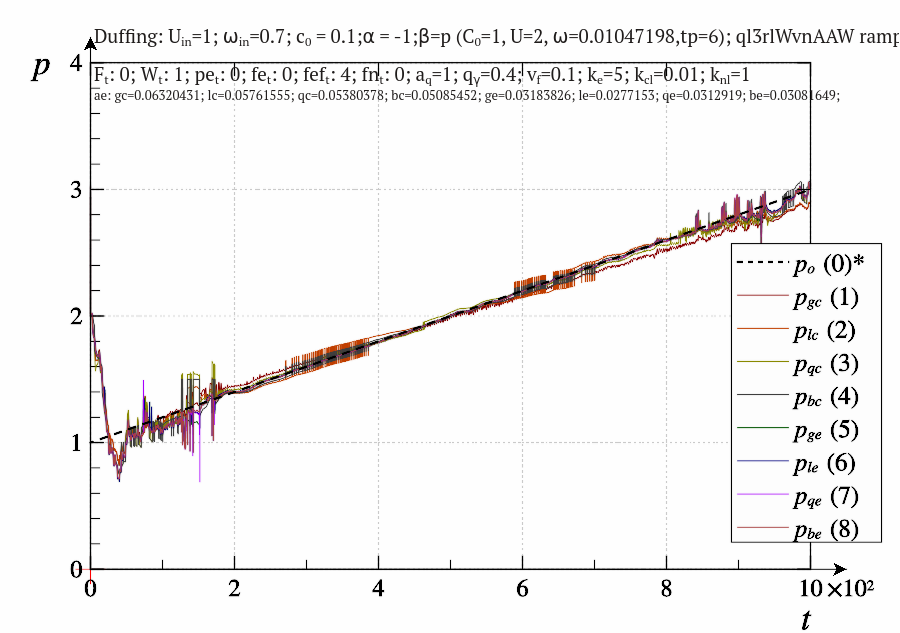
\includegraphics[width=0.49\textwidth]{p/cha/duff/duff_id-p_t_p_ql3rlWvnAAW_ramp.png}
\end{center}
  \caption{Динамика агентов и идентифицируемого значения для системы Дуффинга при условии (\ref{atu:eq:po_t_ramp})}
\label{atu:f:duff_id_ramp}
\end{figure}

% }}}2

\subsection{Влияние параметров системы идентификации на ошибку идентификации для системы Дуффинга}  % {{{2


Зависимости здесь

% }}}2

\subsection{Выводы}  % {{{2

Выводы

% }}}2

% }}}1

% vim: fdm=marker foldlevelstart=2 fdc=4 ft=tex
